\documentclass[11pt]{article}
\usepackage[letterpaper,margin=0.95in]{geometry}
\usepackage[T1]{fontenc}
\usepackage{lmodern}
\usepackage{microtype}
\usepackage{amsmath,amssymb}
\usepackage{graphicx}
\usepackage{booktabs,tabularx,array,multirow}
\usepackage{enumitem}
\usepackage[dvipsnames]{xcolor}
\usepackage{caption}
\usepackage{float}
\usepackage{adjustbox}
\usepackage[hidelinks]{hyperref}
\definecolor{hblue}{HTML}{2a78d6}
\definecolor{boxbg}{HTML}{f4f3ef}
\definecolor{ink2}{HTML}{52514e}
\hypersetup{colorlinks=true,linkcolor=hblue,urlcolor=hblue,citecolor=hblue}
\captionsetup{font=small,labelfont=bf,margin=0.15in}
\setlist{itemsep=2pt,topsep=3pt,parsep=0pt}
\setlength{\parskip}{4pt}
\setlength{\parindent}{0pt}
\graphicspath{{../../../results/}{figs/}}
\newcommand{\keybox}[1]{\par\smallskip\noindent\colorbox{boxbg}{\parbox{\dimexpr\linewidth-2\fboxsep}{\small #1}}\par\smallskip}
\newcommand{\TPR}{\mathrm{TPR}}
\newcommand{\FPR}{\mathrm{FPR}}
\renewcommand{\arraystretch}{1.18}

\sloppy
\usepackage{xurl}

\title{\textbf{Detection-Theoretic Decision Rules for AI-Agent Monitors}\\[4pt]
\large Overall summary of three rounds of experiments, a white-box pilot, and two validity audits}
\date{October 22, 2026 (supersedes the October 21 version)}
\begin{document}
\maketitle
\vspace{-1.2em}

\keybox{\textbf{In one paragraph.} AI-control monitoring has improved its \emph{monitors} (LLM judges, prompts, probes) much more than its \emph{decision layer}: the rule that turns per-step scores into audit decisions. Almost every system takes the maximum over steps and compares it with one global honest-run quantile. Starting from detection theory (Neyman--Pearson, CFAR, CUSUM, sequential tests), we asked three questions:
\begin{enumerate}[leftmargin=1.2em]
\item Do accumulating rules beat max at a matched false-alarm budget?
\item Should thresholds be set per context?
\item Can an attacker who knows the detector game it?
\end{enumerate}
We also ran a white-box pilot that feeds probe scores from an open model into the same decision layer. Over three rounds of experiments, followed by two independent audits that re-derived the headline numbers and corrected several claims, the surviving picture is:
\begin{itemize}[leftmargin=1.2em]
\item \textbf{max} (or top-3 sum) remains the robust default;
\item accumulation helps only in narrow settings;
\item \textbf{CFAR is the wrong per-context rule against an attacker who chooses where to act}, while damage-equalizing (Stackelberg) allocation is better at a 5\% budget;
\item \textbf{LLM rewriting of attacks dominates detector-aware red-teaming}, so an uninformed-rewrite control is essential;
\item a \textbf{probe read on a follow-up question by an open trusted reader beats a cheap LLM monitor at 1\% FPR}, and probe triage nearly doubles detection while calling the LLM on 13\% of steps.
\end{itemize}}

\tableofcontents

\section{What was done}
\begin{enumerate}
\item \textbf{Literature review.} We read 92 arXiv papers in full and 101 lab and community sources (Redwood, Apollo, UK AISI, Anthropic, OpenAI, GDM, METR, security vendors), and wrote a separate review of white-box monitoring. We ranked 10 ideas and ran the top three plus a white-box pilot.
\item \textbf{Infrastructure.} The private repository \texttt{gregkocher/agent-monitor-detection} contains:
  \begin{itemize}
  \item loaders for MonitoringBench, Honest-550, the LinuxArena 12-monitor sweep, aksh-n per-step labels, ScaleAI MRT, persistent-state VibeCoding and MOLE;
  \item a per-step OpenRouter scoring harness (logprob-expected scores, resumable cache);
  \item a detector library calibrated at matched false-alarm budgets;
  \item a spend ledger;
  \item a trusted-reader white-box pipeline on RunPod GPUs.
  \end{itemize}
\item \textbf{Three rounds of experiments} per idea; Section~\ref{sec:ideas} lists them.
\item \textbf{Two independent validity audits.} Each re-derived the headline numbers with its own minimal code and checked calibration leakage, grouping, confounds, onset labels, attack validity, spend matching, selection effects and report/table consistency. A fixer re-analyzed every affected result with corrected methods:
  \begin{itemize}
  \item a single-resampling paired bootstrap clustered by task or account, including calibration noise;
  \item true spend matching;
  \item like-for-like attacker arms;
  \item strict validity;
  \item prompts matched except for the variable under test.
  \end{itemize}
  Corrections are tracked claim by claim in \texttt{results/fixes/corrections.csv} and \texttt{results/audit2/corrections.csv}.
\end{enumerate}

\section{Results at a glance}
\begin{figure}[H]\centering
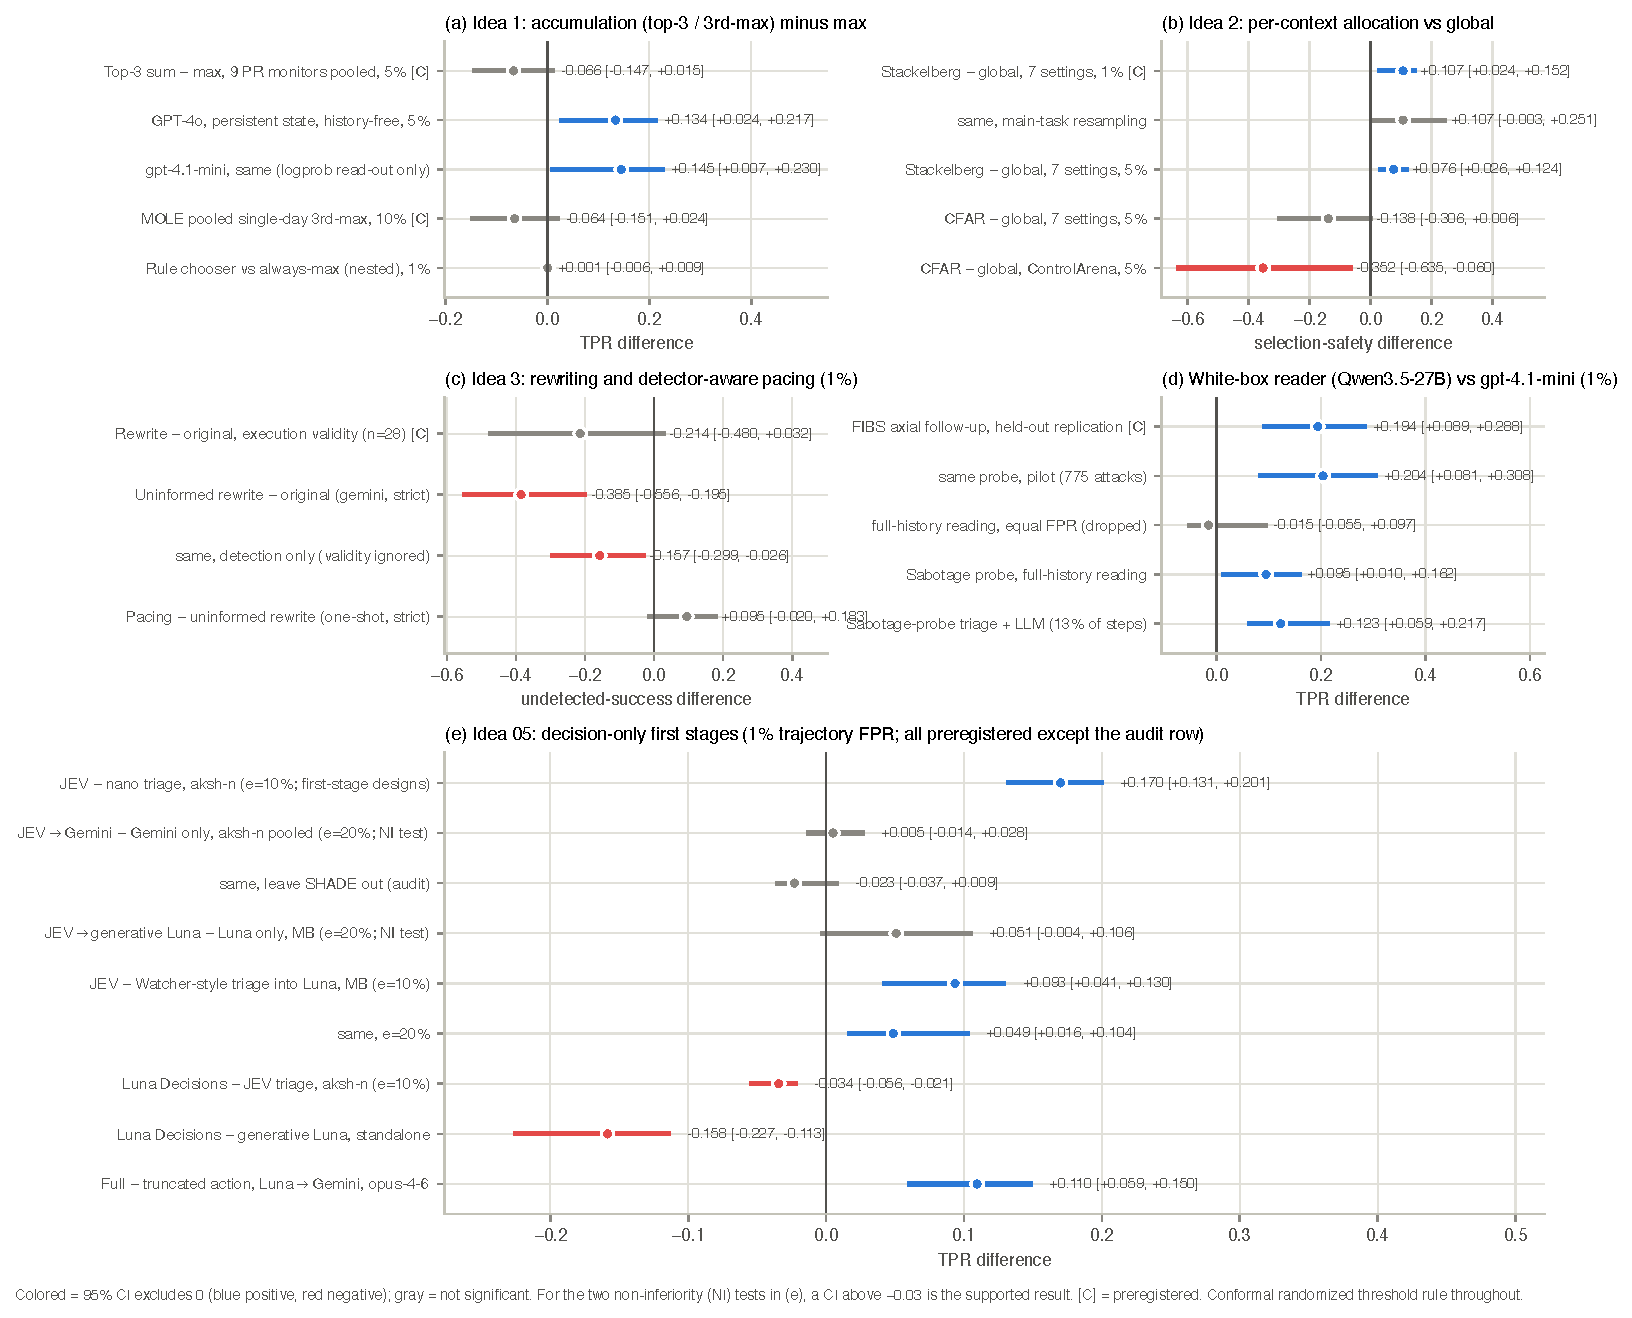
\includegraphics[width=\linewidth]{overview.pdf}
\caption{Audit-verified effects with corrected 95\% CIs. Colored = CI excludes zero; gray = not significant. Sources: \texttt{results/fixes/corrections.csv}, \texttt{results/audit2/corrections.csv}, \texttt{results/t2/tables.md}, \texttt{results/r3\_t3/paired\_contrasts.md}, \texttt{results/wb/tables.md}.}
\end{figure}

\section{The four research directions}\label{sec:ideas}

\subsection{Idea 1: accumulation vs max at a matched budget}
\textbf{Ran.}
\begin{itemize}
\item \textbf{Round 1:} 46 real score-stream sets (aksh-n, LinuxArena sweep, MRT, persistent state), plus a controlled experiment: MonitoringBench re-scored per step by \texttt{gpt-4.1-mini} with full history vs none.
\item \textbf{Round 2:} cross-session re-scoring of persistent state with three new monitor families; MOLE (30-day accounts); a data-driven rule chooser.
\item \textbf{Round 3:} all 8 MOLE corpora under one common monitor, with activity and account-centering controls; long unreset streams; four ``re-flagging'' monitor designs.
\end{itemize}

\textbf{Holds.}
\begin{itemize}
\item Max, 2nd-max and top-3 sum are strong defaults. Textbook sequential tests (CUSUM $k{=}0.5$, Shiryaev--Roberts, e-processes) lose to them on almost every set, partly because most honest steps score exactly 0.
\item Cross-session accumulation with a history-free per-PR GPT-4o monitor: $+0.146$ [0.025, 0.226].
\item On long unreset streams a forgetting rule (CUSUM) beats max: 0.71 vs 0.58 at ARL$_0$ = 100 PRs.
\item On MOLE, no accumulation rule beats max on any of the 8 corpora (pooled 3rd-max $-0.066$ [$-0.156$, 0.023]).
\end{itemize}

\textbf{Weakened.}
\begin{itemize}
\item The \texttt{gpt-4.1-mini} cross-session gain: $+0.145$ [$-0.001$, 0.228].
\item The repeat-spike mechanism: descriptive only once dependence between cells is accounted for.
\end{itemize}

\textbf{Dropped.}
\begin{itemize}
\item The rule chooser's gain ($+0.001$ with nested calibration).
\item ``Accumulators gain more with history''. It was a prompt-instruction confound, and vanishes with prompts matched except for history.
\item The Gemini and Qwen cross-session gains.
\item The round-2 MOLE gain. It was never significant, and was largely an account-activity effect.
\end{itemize}

\subsection{Idea 2: per-context thresholds}
\textbf{Ran.}
\begin{itemize}
\item \textbf{Round 1:} heterogeneity measurement; budget-matched allocation (global, CFAR, Mondrian, partial pooling, max-detection, Stackelberg); context-selecting and poisoning attackers.
\item \textbf{Round 2:} transfer across attack policies and datasets; multi-context poisoning; severity-weighted damage; probing attackers; white-box and strong-monitor panels (E5).
\item \textbf{Round 3:} Watcher-like severity tiers.
\end{itemize}

\textbf{Holds.}
\begin{itemize}
\item Honest-score heterogeneity is large across deployments and small within one. Probe scores are far more context-dependent than LLM scores ($\tau$ up to 3.79 vs $\le0.46$).
\item CFAR is the worst rule against an attacker who chooses its context, and a few alarm-feedback probes break it.
\item Stackelberg beats global at 5\% (0.97 vs 0.89).
\item Partial pooling handles small per-context samples.
\item Watcher-like severity tiers lose 0.06--0.12 to a plain suspicion threshold at 5\% and cannot run at 1\%.
\end{itemize}

\textbf{Weakened or dropped.}
\begin{itemize}
\item The 1\% Stackelberg gain is not established, and the ControlArena 1\% gain is dropped.
\item ``CFAR doubles probe TPR'' was a spend artifact: at equal spend the gain is 1.3--1.5$\times$.
\item Stackelberg fails when fit on different side tasks.
\item The leave-one-context-out poisoning defense breaks when poison is spread across contexts. A frozen trusted reference holds, but over-spends under genuine drift.
\end{itemize}

\subsection{Idea 3: detector-aware attackers}
\textbf{Ran.}
\begin{itemize}
\item \textbf{Round 1:} a \texttt{gpt-4.1} rewriter told the monitor prompt and detector, with \texttt{gpt-4.1-mini} as monitor.
\item \textbf{Round 2:} a strong \texttt{gpt-4.1} monitor; an anti-condensation pacing attacker; an uninformed-rewrite control.
\item \textbf{Round 3:} a different-family rewriter (Gemini 2.5 Pro); a check that fabricated outputs don't leak cues; realized FPR; replay feasibility.
\end{itemize}

\textbf{Holds.}
\begin{itemize}
\item Any LLM rewrite makes attacks easier to catch, whether the rewriter is the monitor's own model family or a different one: $-0.37$ [$-0.55$, $-0.19$] for the Gemini rewriter. About 60\% of that drop is broken attacks; detection only is $-0.14$ [$-0.30$, $-0.03$].
\item Detector-aware pacing shows no significant strategy effect when compared one-shot against one-shot ($+0.087$ [$-0.032$, 0.183]).
\item Max, CUSUM $k{=}1.5$ and top-3 sum hold nominal FPR. The multi-chart OR over-alarms (0.017--0.020 at a nominal 0.01).
\item The covert-adversary $\sqrt{\text{ARL}}$ law is rejected in this setting: detection hinges on single conspicuous steps.
\end{itemize}

\textbf{Retracted.}
\begin{itemize}
\item Round 1's ``aware attacks backfire'' (there was no control).
\item Round 2's ``$+0.21$ pacing gain'' (an adaptive arm was compared with a one-shot control).
\end{itemize}

\subsection{White-box pilot}
\textbf{Ran.}
\begin{itemize}
\item A Qwen3.5-27B trusted reader on two H200 pods, reading each transcript per step or with full history.
\item Signals:
  \begin{itemize}
  \item a synthetic sabotage probe;
  \item Apollo's deception probe;
  \item FAR.AI FIBS probes, read on the step tokens and on a follow-up question;
  \item a J-lens watch-list.
  \end{itemize}
\item All signals passed through the decision layer (decision rules, per-context thresholds, LLM fusion, detector-aware rewrites).
\item Data: MonitoringBench, LinuxArena, and MOLE policy-vs-reader.
\end{itemize}

\textbf{Holds.}
\begin{itemize}
\item The FIBS follow-up probe, read per step, beats \texttt{gpt-4.1-mini} at 1\% FPR: $+0.21$ [0.09, 0.32]. It is the only contrast that survives Holm correction across 18.
\item Sabotage-probe triage plus LLM (13\% of steps) reaches 0.30 vs 0.17 at matched realized FPR.
\item Pre-onset attack steps score like honest steps, so the probe is not leaking the attack in advance.
\end{itemize}

\textbf{Weakened.}
\begin{itemize}
\item The full-history sabotage probe gain ($+0.10$): Holm $p$ 0.22, and present only on one attack agent model.
\item The full-history follow-up probe and the fusions built on it: its threshold does not transfer across tasks (2.05\% realized FPR at a nominal 1\%).
\item The LinuxArena ranking and the round-1 rewrite comparison: their score files were lost in the final pod sync, so they are now unverifiable.
\end{itemize}

\textbf{Not supported.}
\begin{itemize}
\item J-lens watch-list readouts (AUROC $\le$ 0.72).
\item Reading with the agent's own model beating the trusted reader on the sabotage probe.
\end{itemize}

\section{Recommendations for practitioners}
\begin{enumerate}
\item \textbf{Default trajectory rule:} max with a length-aware null where lengths differ; top-3 sum or CUSUM with $k\approx1.5$ as alternatives. Calibrate any OR combination \emph{jointly}, and verify realized FPR on held-out honest runs.
\item \textbf{Accumulate across sessions only after checking} that repeated high scores are informative for your monitor and data. Prefer history-free per-session judgments, and use forgetting rules on long streams.
\item \textbf{Per-context thresholds:}
  \begin{itemize}
  \item measure heterogeneity first;
  \item never use CFAR when attackers can choose contexts;
  \item use Stackelberg (damage-equalizing) allocation fit on attack data that resembles the threat, with shrinkage;
  \item use partial pooling for small samples;
  \item use a trusted frozen reference against poisoning.
  \end{itemize}
\item \textbf{Severity tiers} (Watcher-style) should be validated against an honest hit-rate before being wired in. Rank by suspicion, with one budget-matched threshold per deployment.
\item \textbf{Red-teaming with LLM rewrites} must include an uninformed-rewrite control and strict validity checks; otherwise the rewrite artifact masquerades as a strategy effect.
\item \textbf{White-box:} a probe read on a follow-up question is a cheap, strong complement to LLM monitors, and an efficient triage stage. Probe thresholds are strongly context-dependent, so calibrate per context.
\end{enumerate}

\section{What is new (to our knowledge, per the literature review)}
\begin{itemize}
\item A matched-budget comparison of sequential and anytime-valid statistics vs max on real AI-control score streams. It answers MonitoringBench's stated open question, largely in favor of max.
\item Evidence, with corrected CIs, that cross-session accumulation of history-free judgments can beat max for some monitors. The source paper tested only a failing k-strikes rule.
\item A per-context threshold study for control monitors: CFAR's failure under attack selection, the Stackelberg alternative, poisoning-robust baselines, and Watcher-like severity tiers.
\item Evidence that LLM rewrite artifacts dominate detector-aware red-teaming, and that detector-aware pacing shows no measurable strategy effect once controlled.
\item A trusted-reader white-box pipeline evaluated through the same decision layer, showing a follow-up-question probe beating a cheap LLM monitor at 1\% FPR, and efficient probe triage.
\end{itemize}

\section{Validity process and errata}
The first audit found 2 critical, 9 major and 13 minor issues; the second found 4 major and 10 minor. All point estimates reproduced with independent code. The main corrections relative to the October 21 summary:

\begin{table}[H]\centering\small
\begin{adjustbox}{max width=\linewidth}
\begin{tabular}{@{}llll@{}}
\toprule
Original claim (Oct 21) & Corrected & Verdict & Source\\
\midrule
Cross-session gain $+0.15$ [0.12, 0.17] & GPT-4o $+0.146$ [0.025, 0.226]; gpt-4.1-mini [$-0.001$, 0.228] & holds / weakened & fixes C2\\
Rule chooser $+0.023$ & $+0.001$ [$-0.014$, 0.013] (nested) & dropped & fixes M6\\
Accumulators gain more with history & prompt confound; DiD $\approx 0$ with matched prompts & dropped & fixes M4\\
CFAR doubles probe TPR at 1\% & 1\% not estimable; 1.3--1.5$\times$ at equal spend & dropped / weakened & fixes C1\\
Aware attacks backfire (round 1) & rewrite artifact (control arm) & dropped & fixes M3\\
Pacing vs control $+0.21$ & one-shot vs one-shot $+0.087$ [$-0.032$, 0.183] & weakened (n.s.) & fixes M1\\
Gemini rewrite cost $-0.37$ & detection only $-0.14$ [$-0.30$, $-0.03$] & weakened & audit2 A4\\
MOLE accumulation gain $+0.13$ & never significant; no rule beats max on 8 corpora & dropped & r3\_t1, audit2\\
History-aware follow-up probe lead & threshold over-alarms (2.05\% at 1\%) & weakened & audit2 A1\\
\bottomrule
\end{tabular}
\end{adjustbox}
\end{table}

\section{Budget, compute and artifacts}
\begin{table}[H]\centering\small
\begin{tabular}{@{}lrl@{}}
\toprule
Item & Spend & Notes\\
\midrule
Round 1 (OpenRouter) & \$195.56 & Ideas 1--3 initial experiments\\
Round 2 (OpenRouter) & \$455.61 & Idea 1 \$147.89, Idea 3 \$304.77, white-box \$2.95\\
Round 3 (OpenRouter) & \$294.20 & Idea 1 \$161.36, Idea 2 \$21.82, Idea 3 \$111.02\\
Audit fixes (OpenRouter) & \$25.31 & matched-prompt re-scoring\\
\midrule
\textbf{OpenRouter total} & \textbf{\$970.69} & MATS account; no personal-key spend\\
RunPod GPU & $\approx$\$72 & H200 pods for the white-box reader; all deleted\\
\bottomrule
\end{tabular}
\end{table}
\begin{itemize}
\item \textbf{Repository:} \url{https://github.com/gregkocher/agent-monitor-detection} (private). Code in \texttt{amd/} and \texttt{tracks/}, results in \texttt{results/}, write-ups in \texttt{docs/}.
\item \textbf{Run history:} \texttt{EXPERIMENT\_LOG.md} has the full dated history.
\item \textbf{Detailed reports:} \texttt{docs/reports/01\_Idea1\_Matched\_Budget.pdf}, \texttt{02\_Idea2\_Per\_Context\_Thresholds.pdf}, \texttt{03\_Idea3\_Aware\_Attacker.pdf}, \texttt{04\_WhiteBox\_Pilot.pdf}.
\item \textbf{Literature:} \texttt{docs/research/} has the literature summary, idea ranking and reading cards.
\end{itemize}

\section{Limitations and next steps}
\textbf{Limitations.}
\begin{itemize}
\item \textbf{Weak monitors and small samples.} The re-scored monitors are mostly cheap (\texttt{gpt-4.1-mini}/\texttt{gpt-4.1}). Many attack sets are small (35--150 base attacks), and honest sets are 200--550 runs. Low-FPR estimates are noisy.
\item \textbf{Attacks were not executed.} Rewritten attacks were validated by LLM judge plus target-literal checks only.
\item \textbf{Lost white-box files.} Some white-box score files were lost, and the LinuxArena reader results cannot be re-derived.
\end{itemize}

\textbf{Recommended next steps}, in priority order:
\begin{enumerate}
\item \textbf{Execution replay of attacks} (\$0 API, laptop Docker). The infrastructure works. It needs:
  \begin{itemize}
  \item structured tool calls re-extracted from the source logs;
  \item a rewriter that outputs structured calls.
  \end{itemize}
\item \textbf{White-box follow-ups:}
  \begin{itemize}
  \item a preregistered, Holm-controlled replication of the follow-up probe;
  \item regenerating the lost score files;
  \item a policy-activation arm with account-matched benign sessions.
  \end{itemize}
\item \textbf{Cross-session accumulation} with more monitors and longer real multi-session data, using the corrected bootstrap throughout.
\item \textbf{Stackelberg allocation at 1\%}, with more honest runs per context so 1\% is reachable.
\end{enumerate}
\end{document}
